\section{RF classifier}
\label{sec:intro}

The random forest model has several key hyperparameters, and testing them all simultaneously would require excessive effort and time. Therefore, we fixed the optimal parameters in the sequence described below. Also, to ensure result stability, each test was executed 10 times. The average of 10 results displayed in a graph, and all the confusion matrix represents the best result among those. All training and testing time was measured excluding the codebook generation and vector quantization time; in other words, only the time spent on random forest classification applied on the 256-dimension quantized vectors was measured.
\begin{enumerate}
	\item Number of Trees \& Tree Depth: We tested using an axis-aligned weak learner with the split number fixed at 10.
	\item Split Number (Randomness Parameter): Using the optimal number of trees\&tree depth derived in step 1 and axis-aligned weak learner.
	\item Type of Weak Learner: Using the optimal values for other parameters determined in steps 1 and 2, we tested different weak learners.
\end{enumerate}

%-------------------------------------------------------------------------
\subsection{Number of trees \& The depth of trees}
\label{subsec:Q2_1}
Changing the number of trees and depth, we extracted the result in \cref{fig:q2-fig1}. In the graph, the best accuracy 0.685 occurred at $N \text{(number of trees)} = 250$ and $D\text{ (depth)}=8$, explained as follows:
\begin{itemize}
	\item Number of Trees: A single tree in random forests tends to overfit to data; therefore, we can generalize the model using ensembles of trees. As shown in \cref{fig:q2-fig2}, the test accuracy converges near $N=250$, which is selected as optimal parameter.
	\item Tree Depth: When depth is $D$, maximum of $2^D-1$ nodes are generated. As shown in \cref{fig:q2-fig3}, for a given $N$, test accuracy initially increases with tree depth but later decreases due to overfitting. Notably, the optimal depth $D$ increases with $N$, indicating that a larger $N$ result in less overfitting.
\end{itemize}

\noindent
When $N = \text{(number of trees)}$, $D = \text{(depth)}$ and $\rho = \text{(number of attempts to split per node)}$, the theoretical training/testing time is as below, and our training time results almost align with theoretical predictions as shown in \cref{fig:q2-fig2}, \cref{fig:q2-fig3}. However, since the testing time is generally more than 10 times shorter than the training time, it is sensitive to noise caused by memory loading time. Unlike our expectations, the testing time graph with respect to the value of $D$ is not seem as linear complexity, due to the influence of noise caused by the exponentially increasing memory with tree depth.

\begin{itemize}
	\item Training time: $O(ND\rho \times \text{number of training data})$
	\item Testing time: $O(ND \times \text{number of testing data})$
	\item Space complexity (= Number of nodes): $O(2^{D} \times N)$
\end{itemize}

\begin{figure}
	\centering
	\begin{subfigure}[H]{\linewidth}
		\centering
		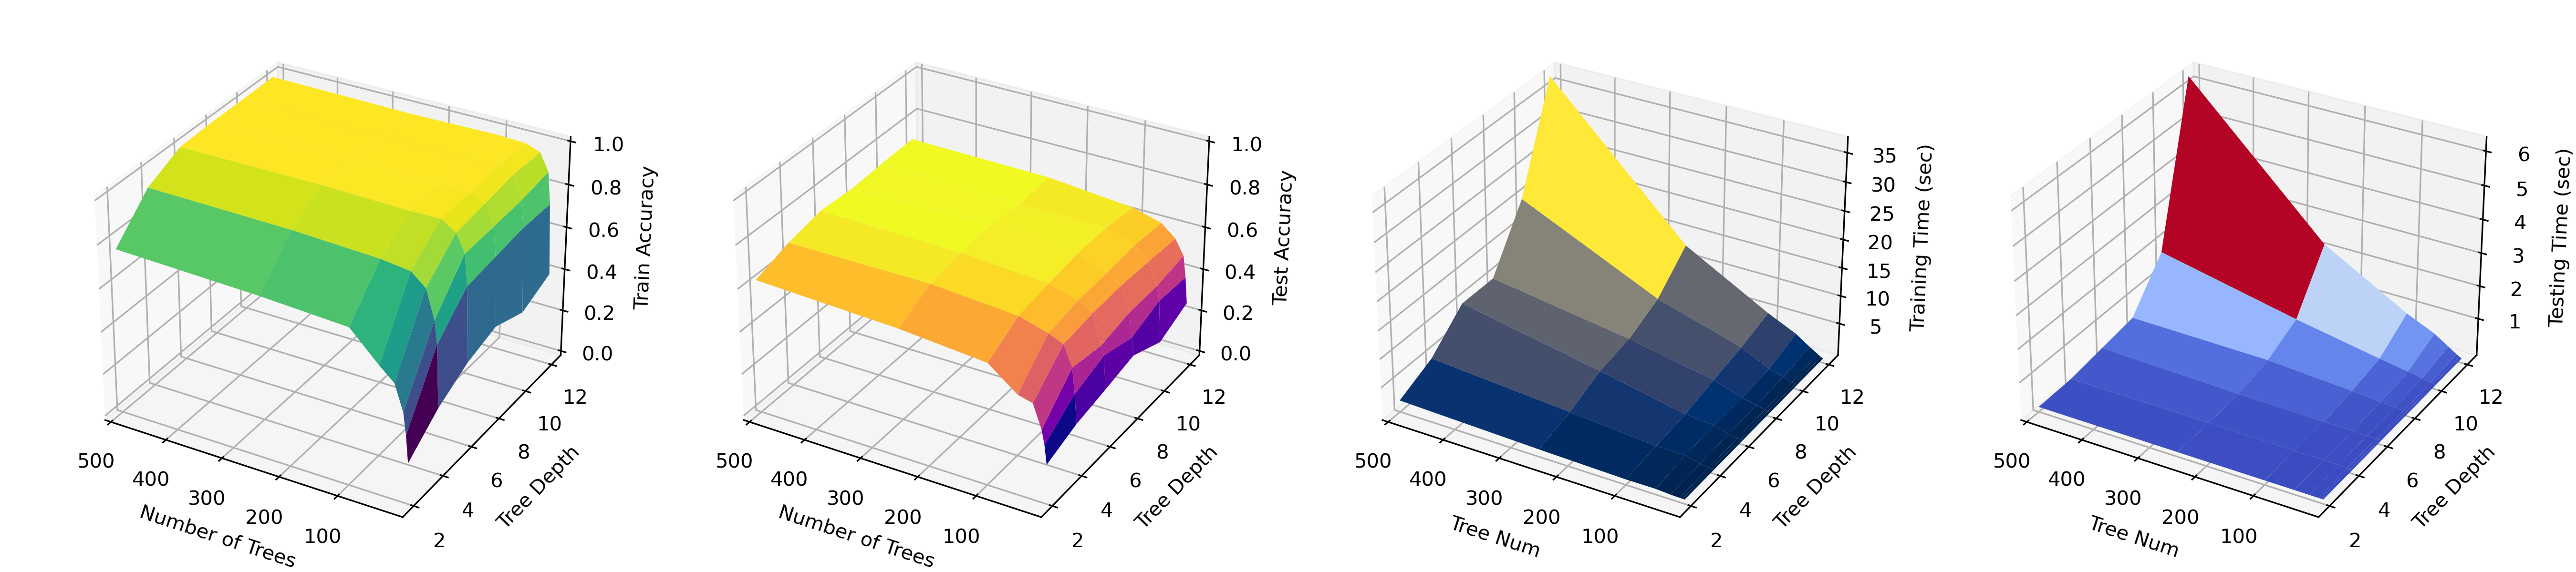
\includegraphics[width=\linewidth]{image/q2-fig1-1.png}
		\caption{Training\&Testing accuracy and time according to the number of tree and the depth of tree}
		\label{fig:q2-fig1}
	\end{subfigure}
	\begin{subfigure}[H]{\linewidth}
		\centering
		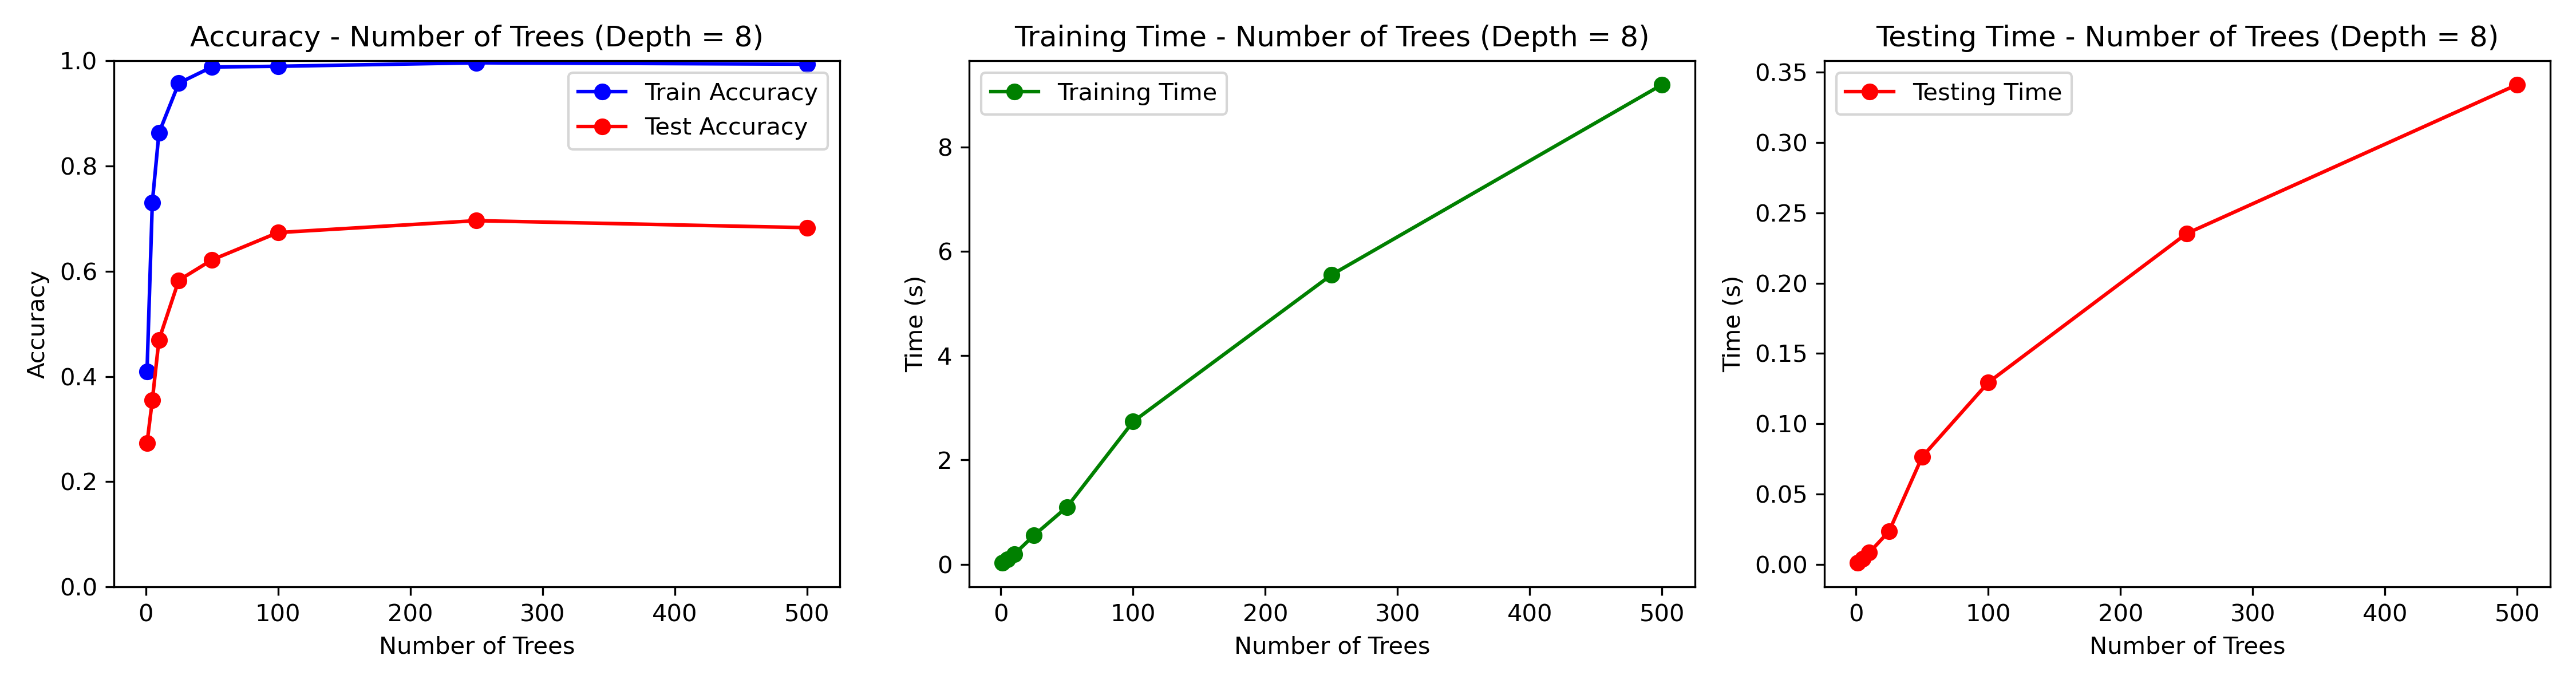
\includegraphics[width=0.8\linewidth]{image/q2-fig2.png}
		\caption{Train\&Test accuracy and time according to the number of tree (D = 8)}
		\label{fig:q2-fig2}
	\end{subfigure}
	\begin{subfigure}[H]{\linewidth}
		\centering
		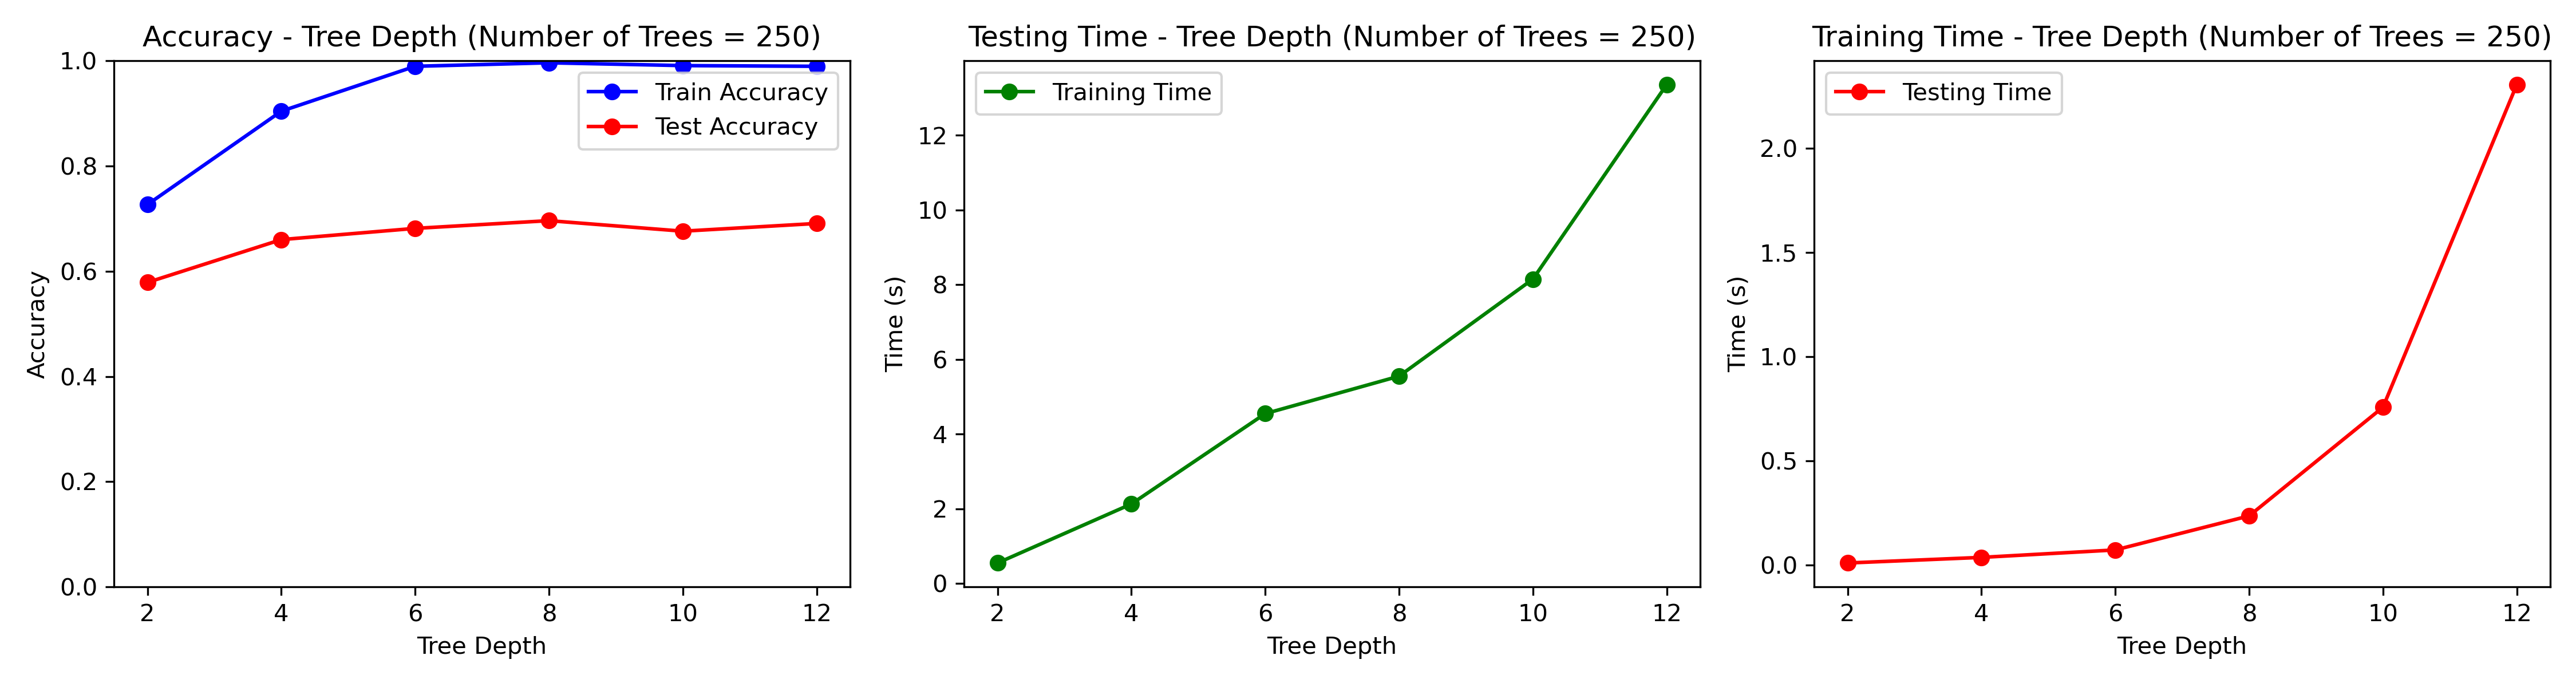
\includegraphics[width=0.8\linewidth]{image/q2-fig3.png}
		\caption{Training\&Testing accuracy and time according to the depth of tree (N = 250)}
		\label{fig:q2-fig3}
	\end{subfigure}
	\caption{Train\&Test accuracy and time according to the number and depth of trees}
\end{figure}
\noindent
Moreover, our code do not utilize parallelization of each tree's growth. Based on theoretical insights from course materials, training each tree in parallel could reduce the time complexity from $O(N)$ to $O(1)$ with respect to the number of trees.

\subsection{Randomness parameter}
We randomly select dimensions and threshold values to create the split function. For each split function, we attempt $\rho$ random splits and choose the one with highest information gain. There is a trade-off in the magnitude of $\rho$ value: If the $\rho$ value is too low, fewer splits are attempted, which reduces similarity between trees but increases the risk of less-optimal split. Conversely, as $\rho$ increases, more various split functions are tested, leading to greater similarity among trees, which decreases the advantage of ensemble multiple trees. As shown in \cref{fig:q2-fig4}, test accuracy initially increases with higher $\rho$ values until $\rho=10$ and then decreases, as expected. Training and testing time is same as the expectation in \cref{subsec:Q2_1}.

\begin{figure}
	\centering
	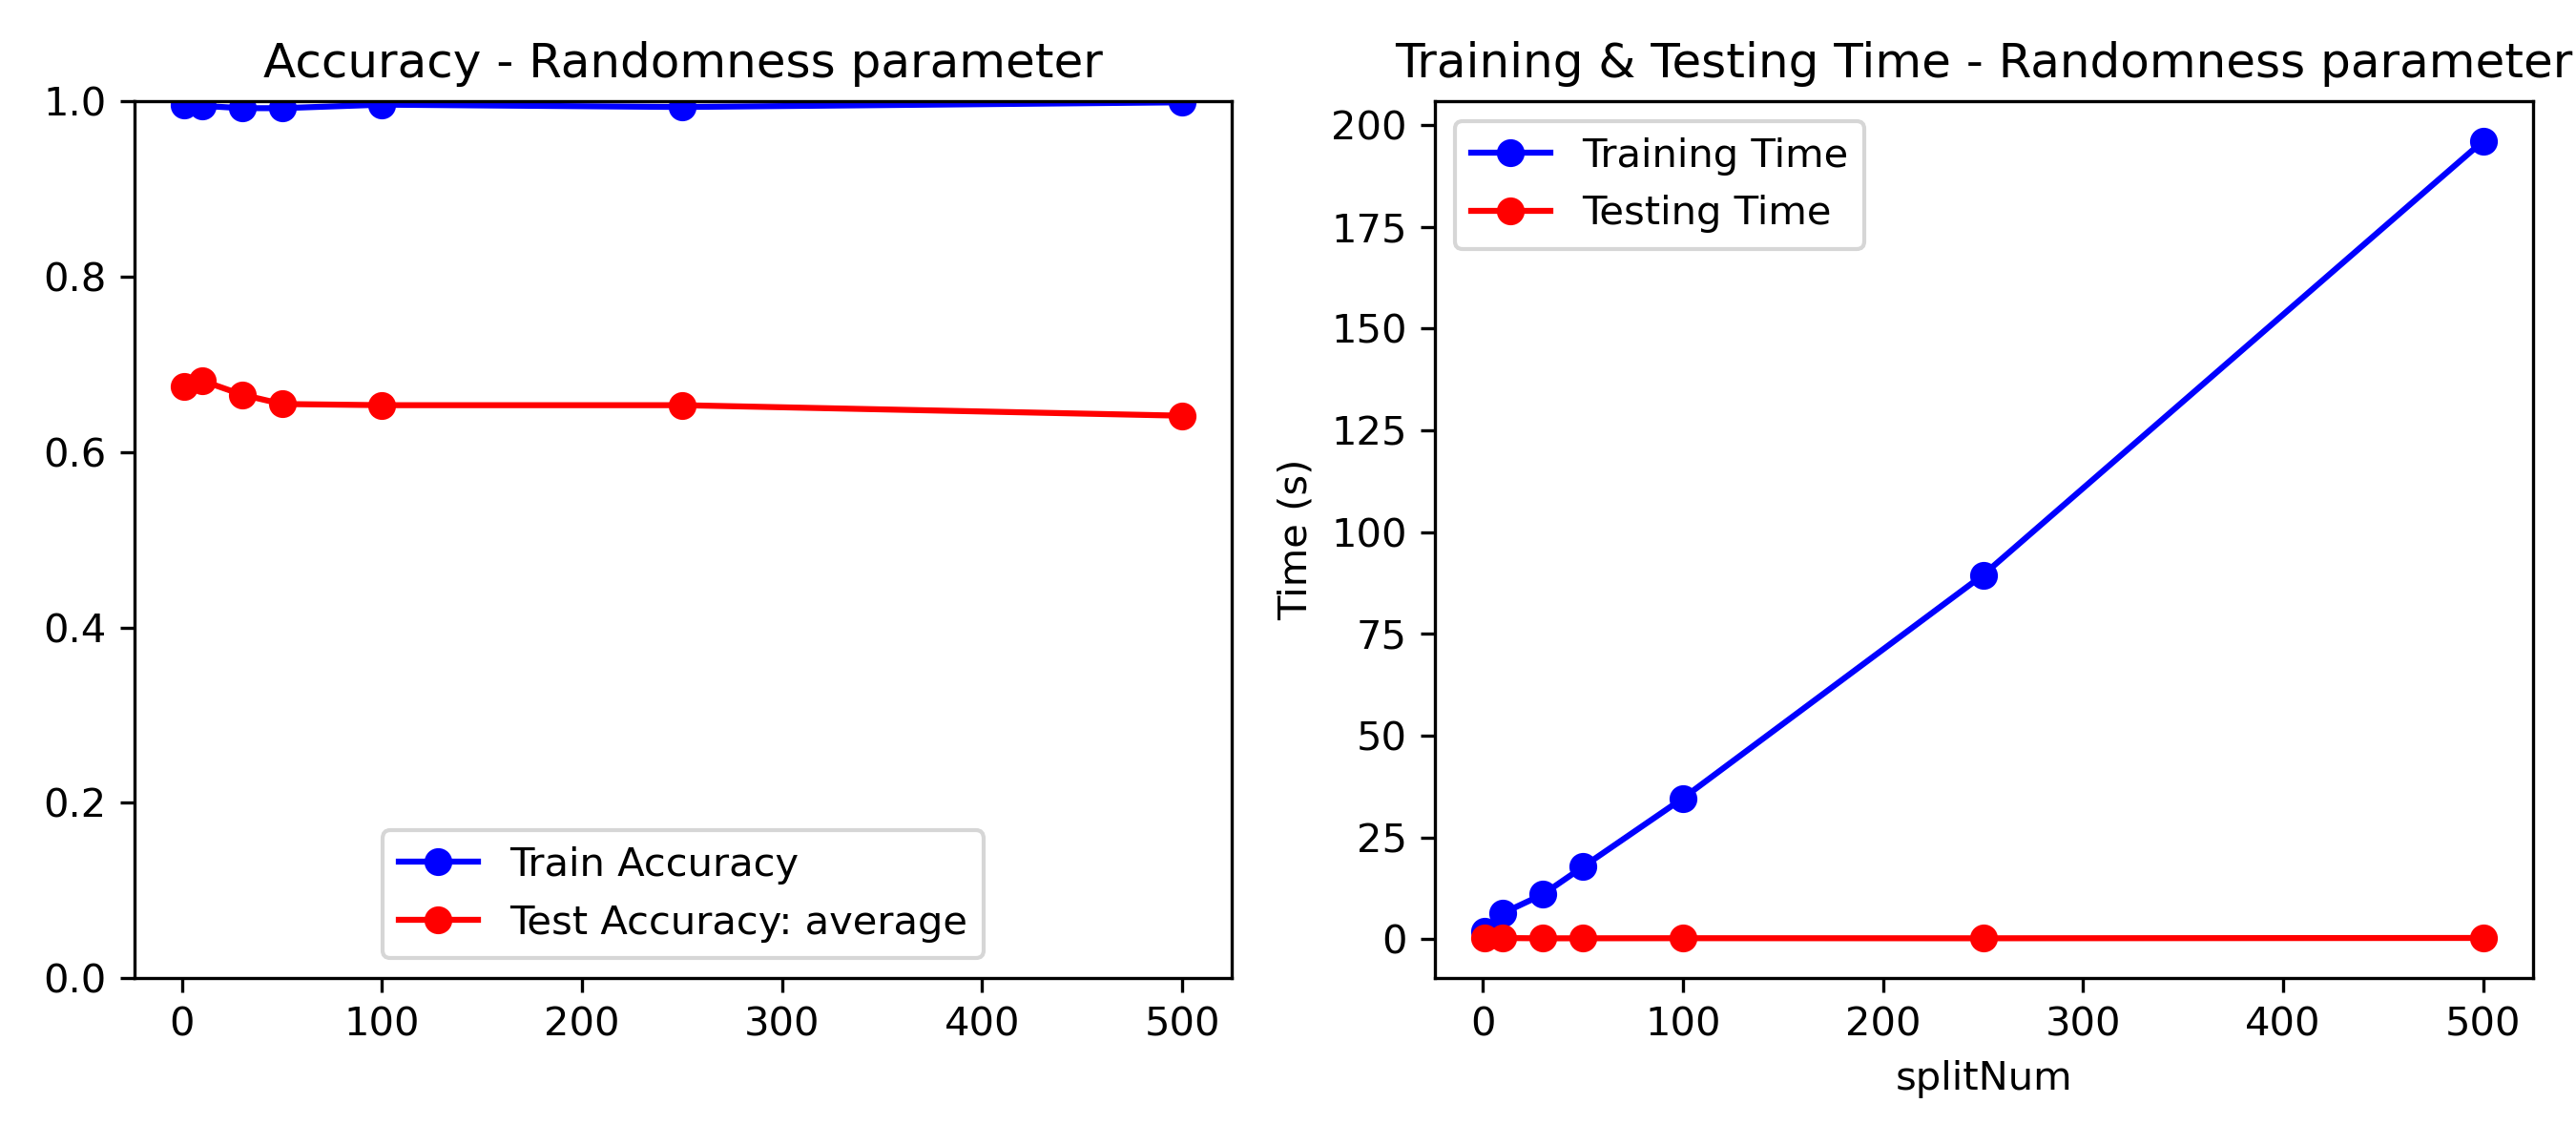
\includegraphics[width=0.55\linewidth]{image/q2-fig4.png}
	\caption{Training\&Testing accuracy and time according to the randomness parameter}
	\label{fig:q2-fig4}
\end{figure}

\subsection{Impact of the vocabulary size on classification accuracy}
We fixed the random forest classification parameters obtained from the previous experiments and varied the K-means vocabulary size. As shown in \cref{fig:q2-fig5}, the vocabulary size used in vector quantization significantly affects both test and train accuracy. As expected, when the value of $K$ is small, because of the insufficient extraction of important features from the images, underfitting occurs, resulting in low training and testing accuracy. Up to $K=16$, train and test accuracy increase rapidly, but beyond that point, the rate of increase for both becomes smaller. Particularly, when $K$ increases from $K=256$ to $K=512$, train accuracy shows a slight improvement, but due to overfitting, test accuracy decreases afterwards. This is because vector quantization extracts unnecessary small details from the images, reducing inner-class vector similarity.

\begin{figure}
	\centering
	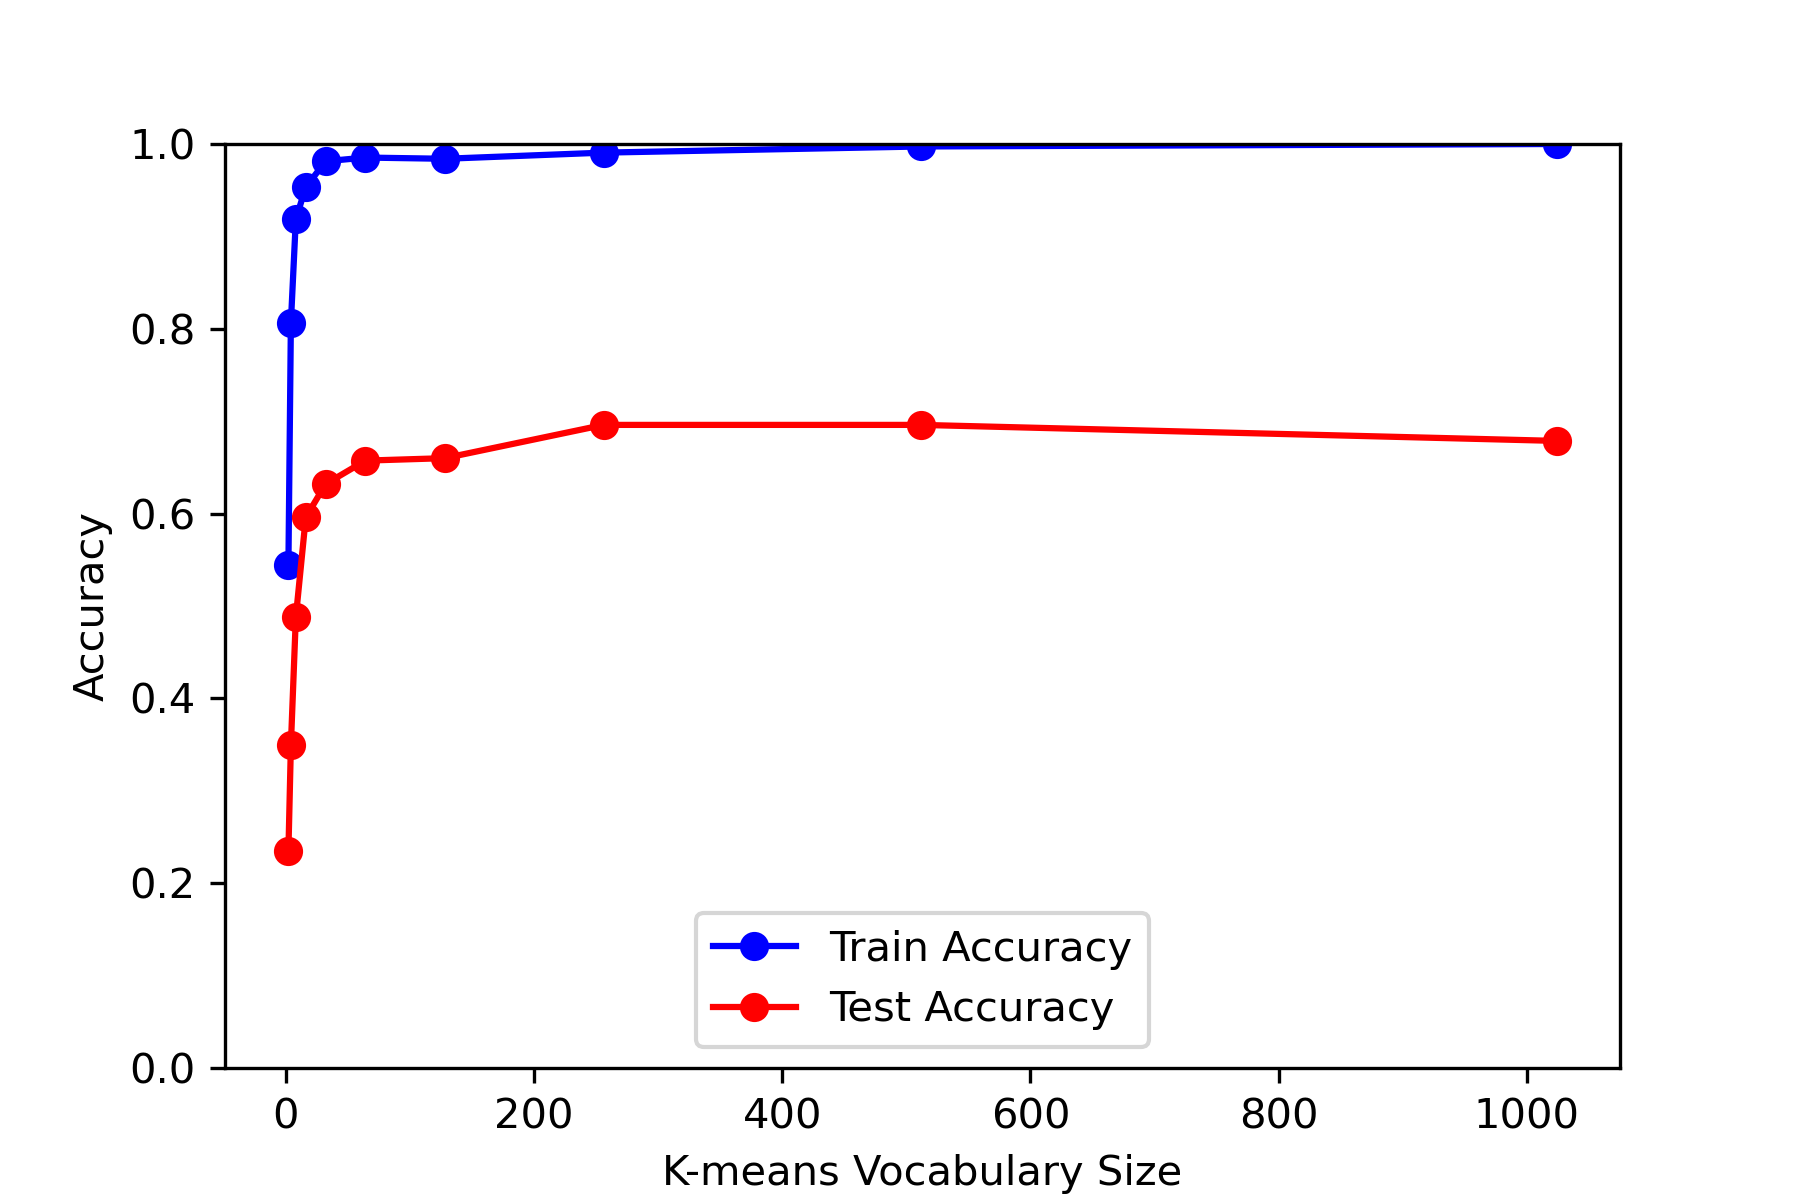
\includegraphics[width=0.4\linewidth]{image/q2-fig5.png}
	\caption{Training\&Testing accuracy according to the K-means vocabulary size}
	\label{fig:q2-fig5}
\end{figure}

\subsection{Impact of the different types of weak-learners}
\cref{fig:q2-fig6} shows the impact of weak learner. As expected, the axis-aligned method provides sufficiently good testing accuracy with shorter training and testing times. However, the two-pixel test achieves 2.13\% better accuracy then axis-aligned under the same parameters. You can see \cref{fig:q2-fig7}, indicating that the two-pixel test has higher information gain per split. Other methods, such as linear and non-linear weak learners, were also tested but omitted from the report due to impractically long training and testing times.

\begin{figure}
	\centering
	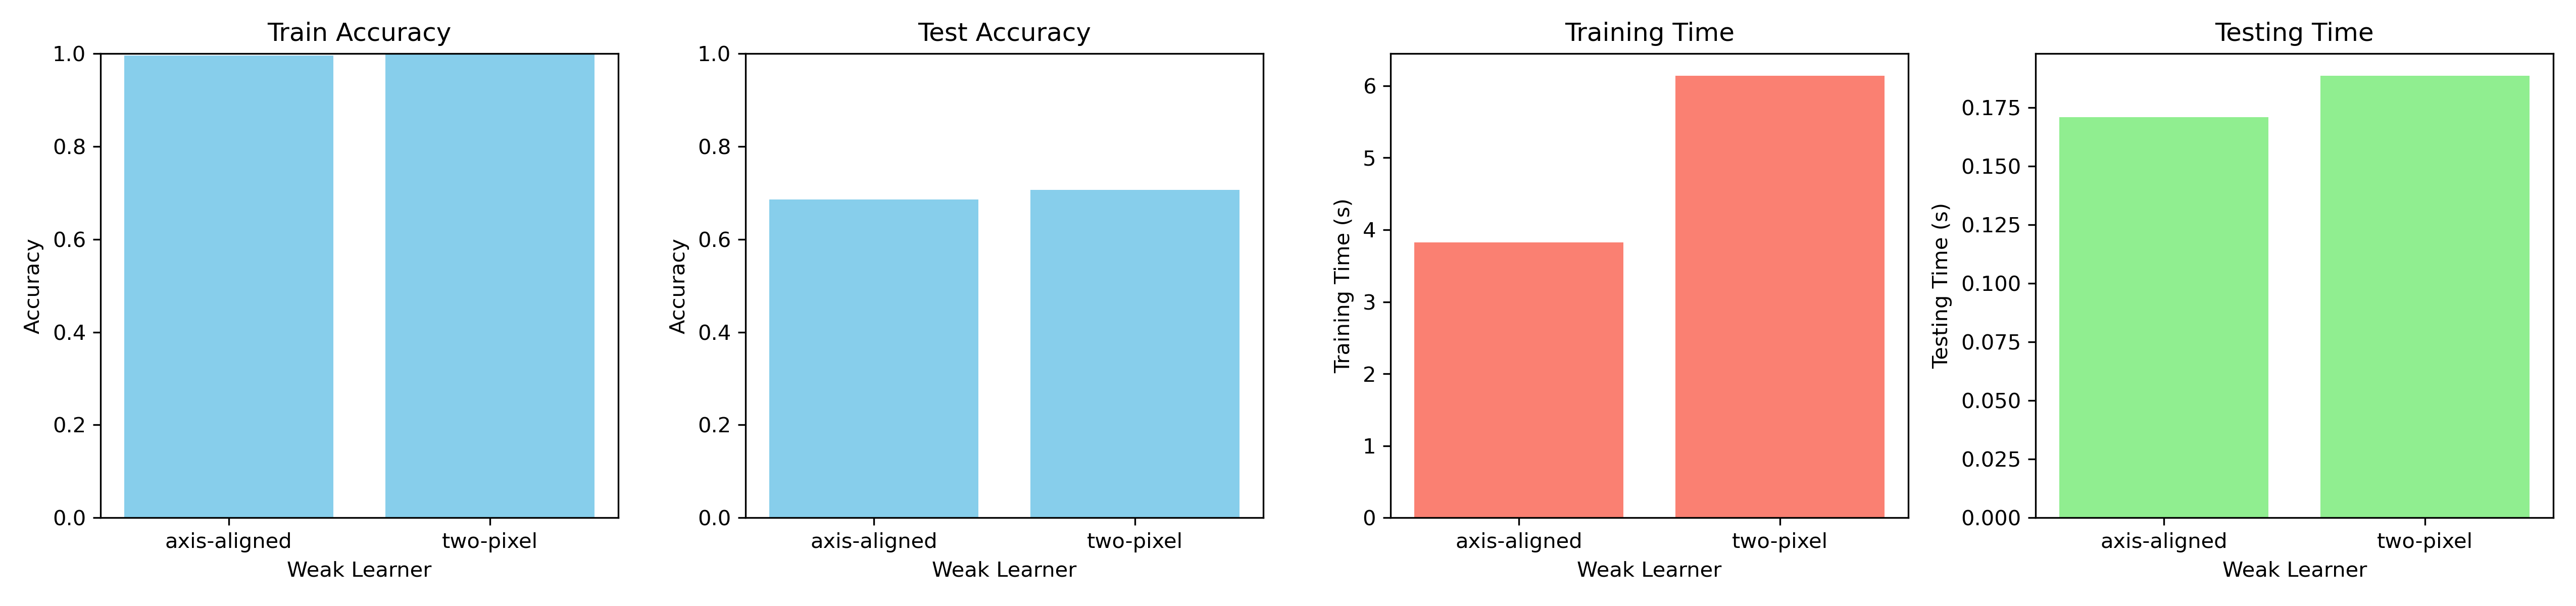
\includegraphics[width=0.8\linewidth]{image/q2-fig6.png}
	\caption{Axis-aligned vs Two-pixel test}
	\label{fig:q2-fig6}
\end{figure}

\begin{figure}
	\centering
	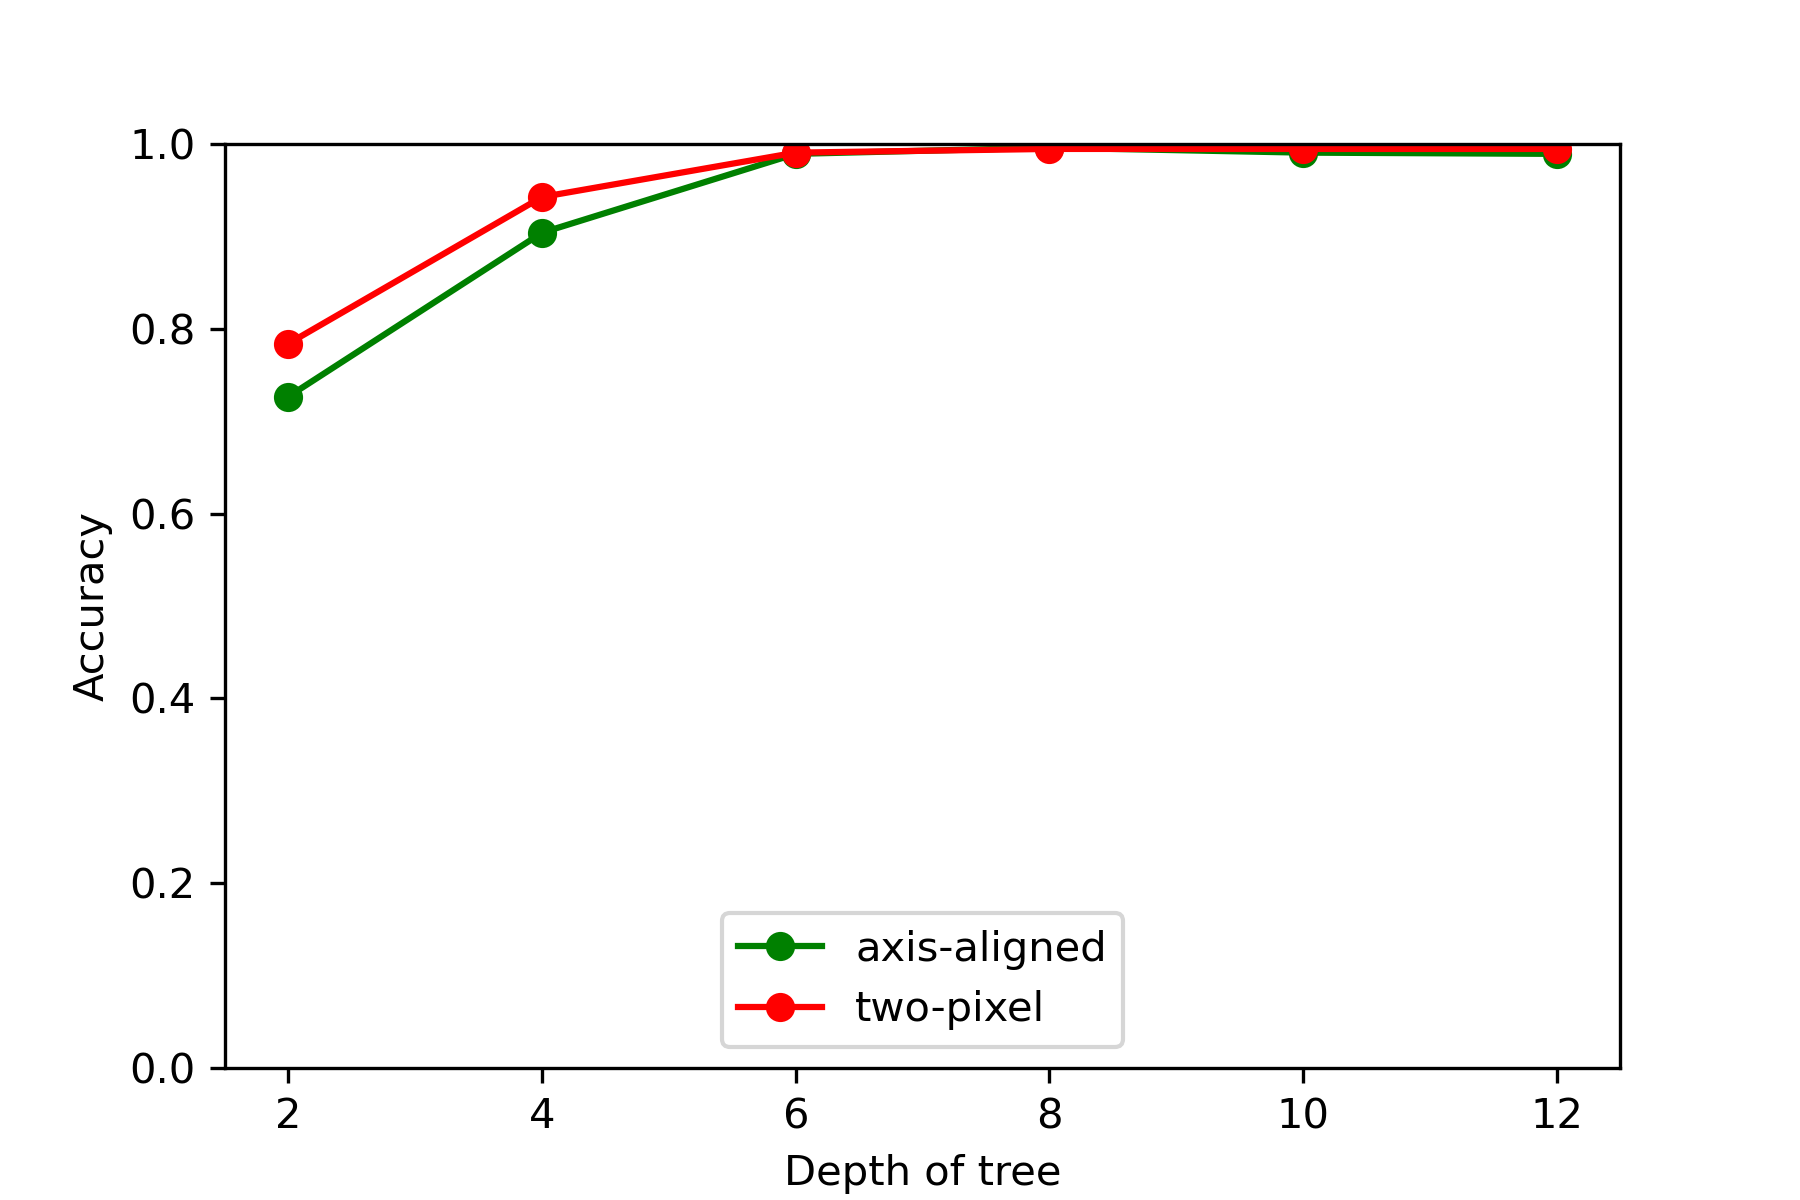
\includegraphics[width=0.4\linewidth]{image/q2-fig7-1.png}
	\caption{Axis-aligned vs Two-pixel test: Train accuracy according to depth of tree}
	\label{fig:q2-fig7}
\end{figure}

The main results' confusion matrix, example success/failures, example node's histogram representing information gain along splitting are written in \cref{subsec:Q2-app1} and \cref{subsec:Q2-app2}